\documentclass[11pt,a4paper]{book}
\usepackage[utf8]{inputenc}
\usepackage[T1]{fontenc}
\usepackage[spanish]{babel}
\usepackage{graphicx}
\usepackage{float}
\usepackage{hhline,colortbl,longtable}
\usepackage{placeins}
\usepackage{multicol}
\usepackage{natbib}
\usepackage{ wasysym }
\bibliographystyle{estilo}
%\bibliographystyle{Science}
\graphicspath{{figures/}}
\author{Miguel Burgos}
\title{Ejemplos de espaciado}

\begin{document}
\begin{figure}
	\centering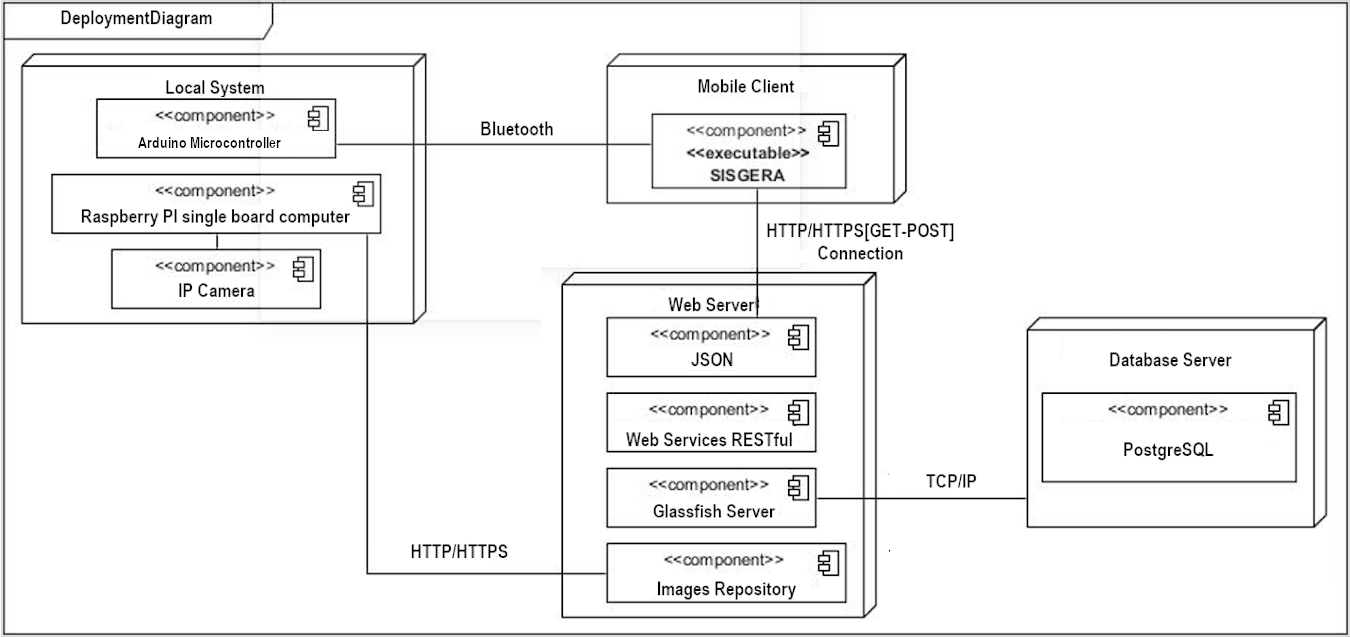
\includegraphics[width=.8\textwidth]{architecture.png}
	\caption{Aquí va el texto que acompaña a la figura}
	\label{fig:cariotipo}
\end{figure}
\end{document}